\chapter{Joshua 12}

\begin{figure}
  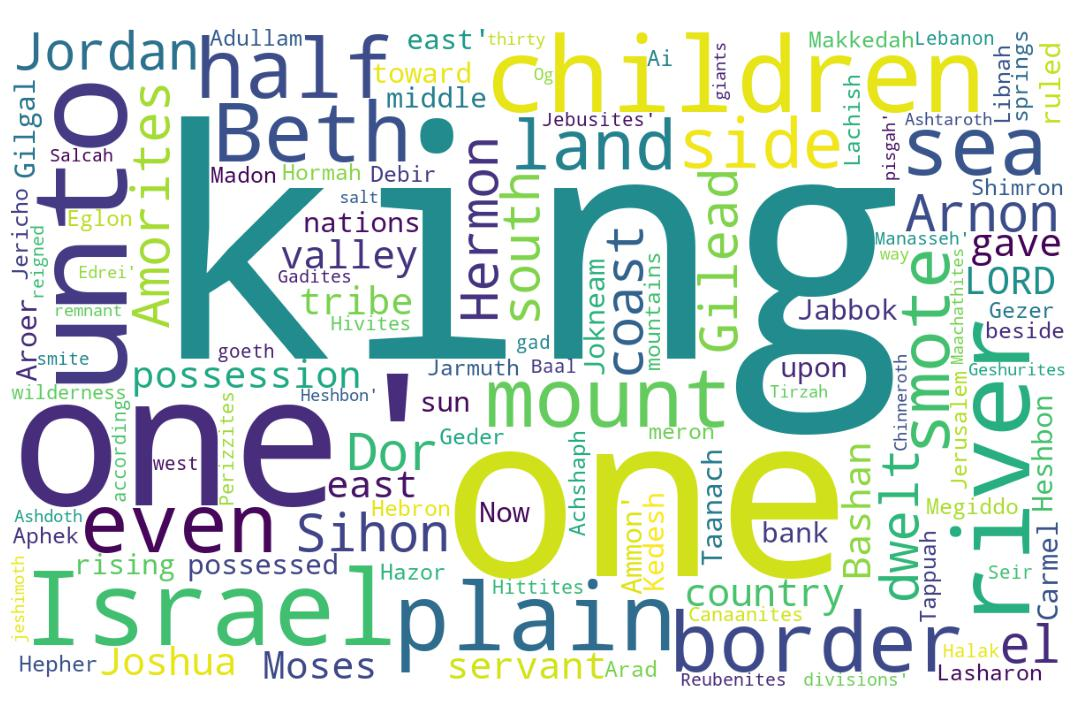
\includegraphics[width=\linewidth]{06OT-Joshua/Joshua12-WordCloud.jpg}
  \caption{Joshua 12 Word Cloud}
  \label{fig:Joshua 12 Word Cloud}
\end{figure}

\marginpar{\scriptsize \centering \fcolorbox{bone}{lime}{\textbf{A RECAP}}\\ (Joshua 12)

\begin{compactenum}[I.][8]

	\item \textbf{These} Ones Defeated  \index[scripture]{Joshua!Jsh 12:01}  (Jsh 12:1, 7) 
	\item \textbf{Tribes} On the Other Side  \index[scripture]{Joshua!Jsh 12:06}  (Jsh 12:6) 
	\item The \textbf{Terrain}  \index[scripture]{Joshua!Jsh 12:08}  (Jsh 12:8) 	
	\item \textbf{Thoughtful} Reflection -- take some time to consider the victories Gad has wrought in your life %\index[scripture]{Joshua!Jsh 12:24}  (Jsh 12:24) 
	\item \textbf{Thirty-One} Kings  \index[scripture]{Joshua!Jsh 12:10-24}  (Jsh 12:10-24) 

\end{compactenum}}





\footnote{\textcolor[cmyk]{0.99998,1,0,0}{\hyperlink{TOC}{Return to end of Table of Contents.}}}\footnote{\href{https://audiobible.com/bible/joshua_12.html}{\textcolor[cmyk]{0.99998,1,0,0}{Joshua 12 Audio}}}\textcolor[cmyk]{0.99998,1,0,0}{Now \fcolorbox{bone}{lime}{these} \emph{are} the kings of the land, which the children of Israel smote, and possessed their land on the other side Jordan toward the rising of the sun, from the river Arnon unto mount Hermon, and all the plain on the east:}
[2] \textcolor[cmyk]{0.99998,1,0,0}{Sihon king of the Amorites, who dwelt in Heshbon, \emph{and} ruled from Aroer, which \emph{is} upon the bank of the river Arnon, and from the middle of the river, and from half Gilead, even unto the river Jabbok, \emph{which} \emph{is} the border of the children of Ammon;}
[3] \textcolor[cmyk]{0.99998,1,0,0}{And from the plain to the sea of Chinneroth on the east, and unto the sea of the plain, \emph{even} the salt sea on the east, the way to Beth-jeshimoth; and from the south, under Ashdoth-pisgah:}\\
\\
\textcolor[cmyk]{0.99998,1,0,0}{And the coast of Og king of Bashan, \emph{which} \emph{was} of the remnant of the giants, that dwelt at Ashtaroth and at Edrei,}
[5] \textcolor[cmyk]{0.99998,1,0,0}{And reigned in mount Hermon, and in Salcah, and in all Bashan, unto the border of the Geshurites and the Maachathites, and half Gilead, the border of Sihon king of Heshbon.}
[6] \textcolor[cmyk]{0.99998,1,0,0}{Them did Moses the servant of the LORD and the children of Israel smite: and Moses the servant of the LORD gave it \emph{for} a possession unto the Reubenites, and the Gadites, and the half \fcolorbox{bone}{lime}{tribe} of Manasseh.}
[7] \textcolor[cmyk]{0.99998,1,0,0}{And \fcolorbox{bone}{lime}{these} \emph{are} the kings of the country which Joshua and the children of Israel smote on this side Jordan on the west, from Baal-gad in the valley of Lebanon even unto the mount Halak, that goeth up to Seir; which Joshua gave unto the tribes of Israel \emph{for} a possession according to their divisions;}
[8] \textcolor[cmyk]{0.99998,1,0,0}{In the \fcolorbox{bone}{lime}{mountains}, and in the \fcolorbox{bone}{lime}{valleys}, and in the \fcolorbox{bone}{lime}{plains}, and in the \fcolorbox{bone}{lime}{springs}, and in the \fcolorbox{bone}{lime}{wilderness}, and in the \fcolorbox{bone}{lime}{south country}; the Hittites, the Amorites, and the Canaanites, the Perizzites, the Hivites, and the Jebusites:}\\
\\
\textcolor[cmyk]{0.99998,1,0,0}{The king of Jericho, one; the king of Ai, which \emph{is} beside Beth-el, one;}
[10] \textcolor[cmyk]{0.99998,1,0,0}{The king of Jerusalem, one; the king of Hebron, one;}
[11] \textcolor[cmyk]{0.99998,1,0,0}{The king of Jarmuth, one; the king of Lachish, one;}
[12] \textcolor[cmyk]{0.99998,1,0,0}{The king of Eglon, one; the king of Gezer, one;}
[13] \textcolor[cmyk]{0.99998,1,0,0}{The king of Debir, one; the king of Geder, one;}
[14] \textcolor[cmyk]{0.99998,1,0,0}{The king of Hormah, one; the king of Arad, one;}
[15] \textcolor[cmyk]{0.99998,1,0,0}{The king of Libnah, one; the king of Adullam, one;}
[16] \textcolor[cmyk]{0.99998,1,0,0}{The king of Makkedah, one; the king of Beth-el, one;}
[17] \textcolor[cmyk]{0.99998,1,0,0}{The king of Tappuah, one; the king of Hepher, one;}
[18] \textcolor[cmyk]{0.99998,1,0,0}{The king of Aphek, one; the king of Lasharon, one;}
[19] \textcolor[cmyk]{0.99998,1,0,0}{The king of Madon, one; the king of Hazor, one;}
[20] \textcolor[cmyk]{0.99998,1,0,0}{The king of Shimron-meron, one; the king of Achshaph, one;}
[21] \textcolor[cmyk]{0.99998,1,0,0}{The king of Taanach, one; the king of Megiddo, one;}
[22] \textcolor[cmyk]{0.99998,1,0,0}{The king of Kedesh, one; the king of Jokneam of Carmel, one;}
[23] \textcolor[cmyk]{0.99998,1,0,0}{The king of Dor in the coast of Dor, one; the king of the nations of Gilgal, one;}
[24] \textcolor[cmyk]{0.99998,1,0,0}{The king of Tirzah, one: all the kings thirty and one.}